% !TEX TS-program = pdflatex
\documentclass[11pt, letterpaper]{article}

%% Packages
\usepackage[utf8]{inputenc}
\usepackage[margin=1in]{geometry}
\usepackage{setspace}
\usepackage{hyperref}
\usepackage{parskip}
\usepackage{mathtools}
\usepackage{amssymb}
\usepackage[figurewithin=section]{caption}
\usepackage{float}

%% Document Setup
\pagestyle{plain}
\onehalfspacing
\numberwithin{equation}{section}
\begin{document}

%% First Page
\title{Design of Path Following Controller for Mobile Robot}
\author{Raj Patel}
\date{November 23, 2020}
\maketitle
\tableofcontents
\newpage

%% Introduction
\section{Introduction}

The line following controller for a mobile robot iteratively finds a line that both is perpendicular to the desired linear path and intersects the position of the robot. Given by geometric constraints, the shortest distance between a line and a point is found on another line that satisfies both said properties. Extrapolating this geometric principle to a nonlinear path, there exists multiple such lines that both are perpendicular to the nonlinear path and intersect the position of the robot. To solve the path following problem for nonlinear paths, the line following controller must be adjusted to (1) take into account the changing direction of the path and (2) minimize the Euclidean distance function in place of solving a linear dot product.

In this paper, a path following controller for a mobile robot is derived and demonstrated. In Section \ref{sec:tech_app}, a detailed derivation of the path following controller is shown. Theoretically, the path following controller would work for any path defined by a continuous function. In Section \ref{sec:results}, the results of the path following controller for a given path and several initial conditions are discussed.

%% Technical Approach
\section{Technical Approach}
\label{sec:tech_app}

%% Unicycle Model
\subsection{Unicycle Model}

In this demonstration, a planar mobile robot with unicycle model will be used. Measurements will be taken with respect to the inertial frame. The unicycle model is defined as
\begin{gather}
    \dot{x} = v \cos(\theta) \text{ ,} \\
    \dot{y} = v \sin(\theta) \text{ ,} \\
    \dot{\theta} = \omega \text{ ,}
\end{gather}

where $(x, y)$ is the position of the robot, $\theta$ is the orientation of the robot, $v$ is the linear velocity of the robot, and $\omega$ is the angular velocity of the robot.

\pagebreak

%% Open-Loop Dynamics
\subsection{Open-Loop Dynamics}

To follow a given path, the distance between the robot and the path must be minimized to the desired distance, and the angular difference between the orientation of the robot and the direction of the path must be minimized to $0$. For this controller design, the robot will assume a constant speed. The open-loop dynamics are defined as
\begin{gather}
    v = v_f \\
    \dot{\rho} = - v \cos(\frac{\pi}{2} - \phi) = -v \sin(\phi) \text{ ,} \\
    \phi = \theta_o - \theta \text{ ,} \\
    \dot{\phi} = \dot{\theta}_o - \dot{\theta} = \dot{\theta}_o - \omega = -v u \text{ ,} \\
    \omega = \dot{\theta}_o + v u \text{ ,}
\end{gather}

where $v$ is the linear velocity of the robot, $\rho$ is the shortest distance between the robot and the path, $\theta$ is the orientation of the robot, $\theta_o$ is the direction of the path, $\omega$ is the angular velocity of the robot, $\phi$ is the angular difference between $\theta$ and $\theta_o$, and $u$ is the control input.

%% General Path Constraints
\subsection{General Path Constraints}

A derivation of the closed-loop forms of parameters is necessary for real-time operation of the controller:
\begin{gather}
    y = f(x)  \text{ ,} \\
    f'(x) = \frac{d}{dx} f(x) \text{ ,} \\
    f''(x) = \frac{d^2}{dx^2} f(x) \text{ ,} \\
    \overrightarrow{p}(x) = \begin{bmatrix} x \\ y \end{bmatrix} = \begin{bmatrix} x \\ f(x) \end{bmatrix} \text{ ,} \\
    q_R(t) = \begin{bmatrix} x_R \\ y_R \end{bmatrix} \text{ ,}
\end{gather}
\begin{gather}
    d(x) = \| q_R(t) - \overrightarrow{p}(x) \| = \sqrt{(x_R - x)^2 + (y_R - f(x))^2} \\
    x_{d_\text{extrema}}(t) = \{x | \frac{d}{dx} d(x)^2 = 0, x \in \mathbb{R} \}  \text{ ,} \\
    \rho(t) = \min (\{d(x_{d_\text{extrema}}(t))\}) \text{ ,} \\
    x_{d_{\min}}(t) = x | \rho = d(x) \text{ ,}
\end{gather}
\begin{gather}
    \overrightarrow{v}(x) = \frac{d}{dx}\overrightarrow{p}(x) = \begin{bmatrix} 1 \\ f'(x) \end{bmatrix} \text{ ,} \\
    \hat{T}(x) = \frac{\overrightarrow{v}(x)}{\| \overrightarrow{v}(x) \|}
               = \begin{bmatrix}
                 \frac{1}{\sqrt{1 + f'(x)^2}} \\[1em]
                 \frac{f'(x)}{\sqrt{1 + f'(x)^2}}
                 \end{bmatrix} \text{ ,} \\
    \theta_o(t) = \arctan(\frac{T_y(x_{d_{\min}}(t))}{T_x(x_{d_{\min}}(t))}) = \arctan(\dot{f}(x_{d_{\min}}(t))) \text{ ,} \\
    \dot{\theta}_o(t) = \frac{d}{dt}\theta_o(t) = \frac{\ddot{f}(x_{d_{\min}}(t))}{1 + \dot{f}(x_{d_{\min}}(t))^2} \text{ ,}
\end{gather}

where $y, f(x), \overrightarrow{p}(x)$ are the (same) desired path, $t$ is the current iteration, $q_R(t)$ is the position of the robot at iteration $t$, $d(x)$ is the Euclidean distance between the robot and the path, $x_{d_\text{extrema}}(t)$ is the set of all local extrema of distances between the robot and the path, $\rho(t)$ is the shortest distance given by the minima in set $x_{d_\text{extrema}}(t)$, $x_{d_{\min}}(t)$ is the x-coordinate of the point on the path that results in $\rho$, $\hat{T}(x)$ is the unit tangential vector of the path, and $\theta_o(t)$ is the direction of the curve at the point of shortest distance to the robot at iteration $t$.

%% Closed-Loop Dynamics
\subsection{Closed-Loop Dynamics}

Proportional feedback control is used to iteratively adjust $\rho$ and $\phi$. The controller is designed to incorporate knowledge of the desired path, the direction of the path, and the velocity and acceleration of the path. The closed-loop dynamics are given by
\begin{gather}
    u = -k_\rho(\rho - \rho_o) - k_\phi(\theta - \theta_o) \text{ ,} \\
    v = v_o \text{ ,} \\
    \dot{\rho} = -v_o \sin(\phi) \text{ ,} \\
    \dot{\phi} = -v_o(-k_\rho(\rho - \rho_o) - k_\phi(\theta - \theta_o)) \text{ ,} \\
    \omega = \frac{\ddot{f}(x_{d_{\min}})}{1 + \dot{f}(x_{d_{\min}})^2} + v_o (-k_\rho(\rho - \rho_o) - k_\phi(\theta - \theta_o)) \text{ ,}
\end{gather}

where $u$ is the control input, $\rho$ is the shortest distance between the robot and the path, $v$ is the linear velocity of the robot, $v_o$ is the desired constant speed of the robot, $\rho_o$ is the desired distance between the robot and the path, $k_\rho$ is the proportional gain for $\rho$, $\theta$ is the orientation of the robot, $\theta_o$ is the direction of the path, $\phi$ is the angular difference between $\theta$ and $\theta_o$, $k_\phi$ is the proportional gain for $\phi$, $\omega$ is the angular velocity of the robot, $x_{d_{\min}}$ is the x-coordinate of the point on the path that results in $\rho$, and $f(x)$ is the desired path.

\pagebreak

%% Stability
\subsection{Stability}

Stability can be analyzed through the linearization of $\dot{\rho}$ and $\dot{\phi}$:
\begin{gather}
    \lim_{x \rightarrow 0} \cos(x) \approx 1 \text{ ,} \\
    \lim_{x \rightarrow 0} \sin(x) \approx x \text{ ,} \\
    \dot{\rho} \approx -v_o \phi \text{ ,} \\
    \dot{\phi} = -v_o(-k_\rho(\rho - \rho_o) - k_\phi(-\phi)) \text{ ,} \\
    \begin{bmatrix} \dot{\rho} \\ \dot{\phi} \end{bmatrix} = \begin{bmatrix} 0 & -v_o \\ v_o k_\rho & -v_o k_\phi \end{bmatrix} \begin{bmatrix} \rho - \rho_o \\ \phi \end{bmatrix} \text{ ,} \\
    A = \begin{bmatrix} 0 & -v_o \\ v_o k_\rho & -v_o k_\phi \end{bmatrix} \text{ ,} \\
    {cp}_A = \det(\lambda I_2 - A) = \lambda^2 + k_\phi v_o \lambda + k_\rho v_o^2 \text{ ,} \\
    \lambda_A = \{\text{roots } {cp}_A \} = v_o \frac{-k_\phi \pm \sqrt{k_\phi^2 - 4 k_\rho}}{2} \text{ ,} \\
    \intertext{For the system poles to be on left-half of complex plane:}
    k_\phi > 0 \text{ ,} \\
    k_\rho > 0 \text{ ,} \\
    \intertext{Further, for the system poles to be real:}
    k_\phi^2 > 4 k_\rho \text{ ,}
\end{gather}

where $\rho$ is the shortest distance between the robot and the path, $v_o$ is the desired constant speed of the robot, $\phi$ is the angular difference between $\theta$ and $\theta_o$, $k_\rho$ is the proportional gain for $\rho$, $\rho_o$ is the desired distance between the robot and the path, $k_\phi$ is the proportional gain for $\phi$, $A$ is a state space matrix of the linearized system, ${cp}_A$ is the characteristic polynomial of the linearized system, and $\lambda_A$ is the set of eigenvalues of the linearized system.

\pagebreak

%% Results
\section{Results}
\label{sec:results}

The parameters had been tuned to optimize results for a specific path:
\begin{gather}
    v_o = 1.2 \text{ ,} \\
    \text{acc} = 1 \text{ ,} \\
    \text{turn\_rt\_lim} = 2.3 \text{ ,} \\
    \text{frame\_shift} = 0.2 \text{ ,} \\
    k_\rho = 0.7 \text{ ,} \\
    k_\phi = \sqrt{4 k_\rho} + 0.2 \text{ ,} \\
    \rho_o = 0.2 \text{ ,} \\
    f(x) = 0.01x^5 - 0.27x^3 + 0.14x^2 + 1.2x - 3 \text{ ,}
\end{gather}

where $v_o$ is the desired constant speed of the robot, acc is the acceleration of the robot, turn\_rt\_lim is the limit of the wheel turning rate of the robot, frame\_shift is the shift difference of the robot's coordinate frame based on the shifted reference point model, $k_\rho$ is the proportional gain for $\rho$, $k_\phi$ is the proportional gain for $\phi$, $\rho_o$ is the desired distance between the robot and the path, and $f(x)$ is the desired path.

These parameters were used consistently for all of the simulations discussed later. $\rho_o$ is consistently nonzero to simulate convergence to a desired distance from an obstacle or wall. The robot was able to converge to the path using the path following controller for many initial conditions. The only parameter changed between each simulation run was the initial condition of the robot.

The initial condition of the robot is given in the form
\begin{equation}
    x(0) = \begin{bmatrix} x(0) \\ y(0) \\ \theta(0) \end{bmatrix}
\end{equation}

\pagebreak

%% Controller Success
\subsection{Controller Success}

In this subsection, the initial conditions discussed are
\begin{gather}
    x_1 = \begin{bmatrix} -4 \\ 2 \\ \frac{\pi}{4} \end{bmatrix} \\
    x_2 = \begin{bmatrix} 0 \\ 2 \\ \frac{-\pi}{4} \end{bmatrix}
\end{gather}

Figure \ref{fig:sim_nr_extr_pth2} and Figure \ref{fig:sim_cent} both show that the robot converges to the desired path from its initial condition. Near sharper turns, using the path following controller, the robot is capable of adjusting and re-converging to the desired path.

\begin{figure}[H]
	\begin{center}
		\includegraphics[height=0.3\textheight, width=0.5\textwidth]{images/sim_nr_extr_pth2.png}
		\caption{Simulation Plot of Desired Path and Robot Path with Initial Condition $x_1$.}
		\label{fig:sim_nr_extr_pth2}
	\end{center}
\end{figure}

\begin{figure}[H]
	\begin{center}
		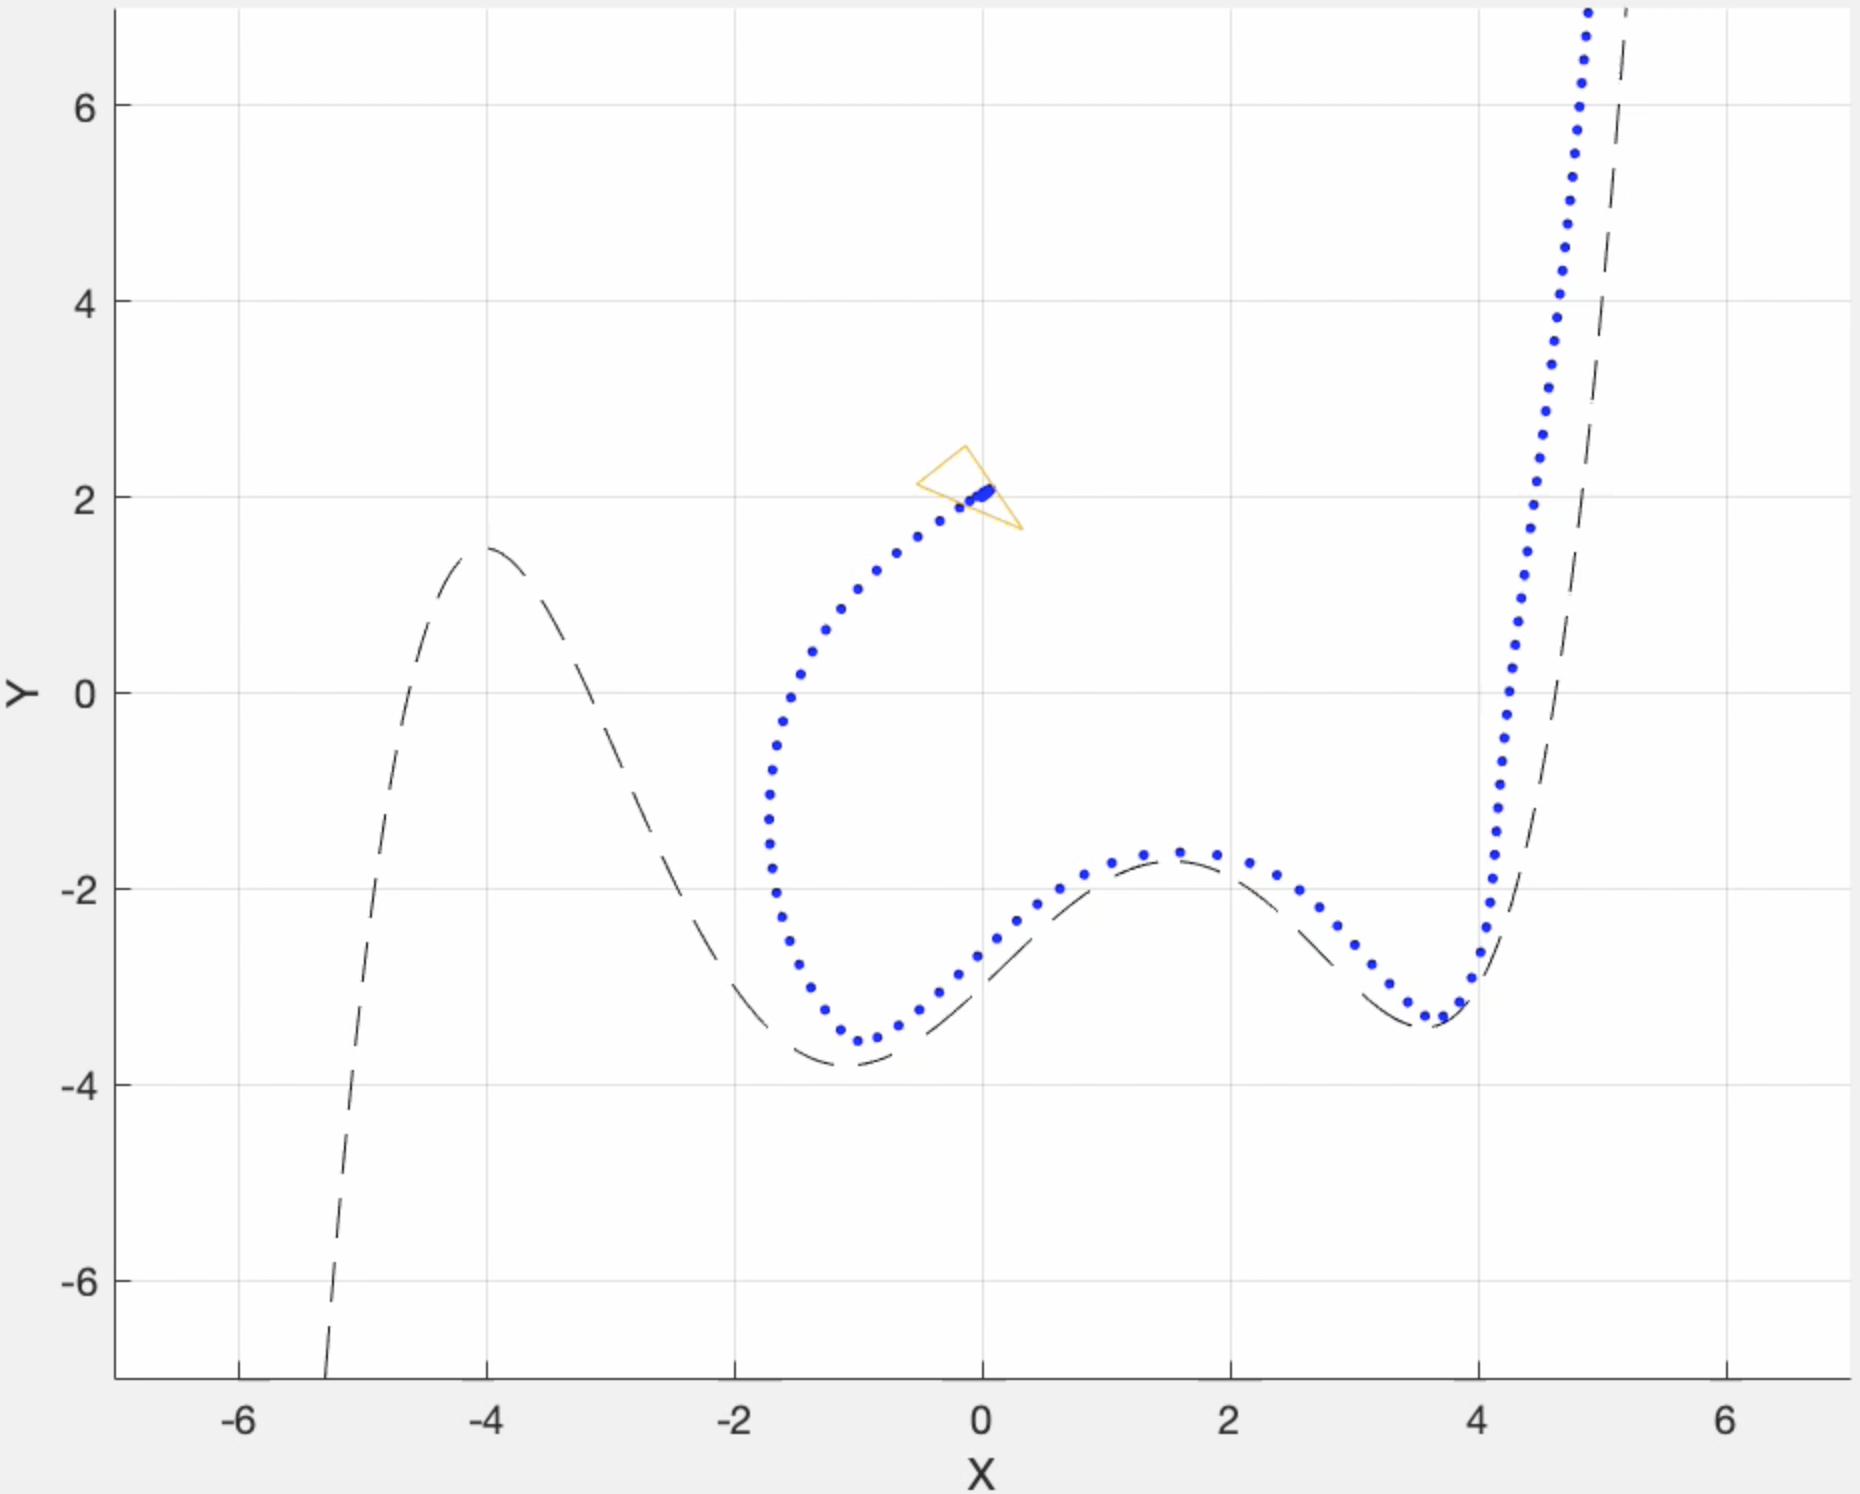
\includegraphics[height=0.3\textheight, width=0.5\textwidth]{images/sim_cent.png}
		\caption{Simulation Plot of Desired Path and Robot Path with Initial Condition $x_2$.}
		\label{fig:sim_cent}
	\end{center}
\end{figure}

%% Controller Semi-Failure
\subsection{Controller Semi-Failure}

In this subsection, the initial conditions discussed are
\begin{gather}
    x_3 = \begin{bmatrix} -6 \\ 4 \\ \frac{\pi}{3} \end{bmatrix} \\
    x_4 = \begin{bmatrix} -4 \\ 2 \\ 0 \end{bmatrix}
\end{gather}

Around regions of higher curvature of the desired path, the robot is more susceptible to getting to close to the desired path, or even touching or shortly crossing over the desired path. Since there is no knowledge of future positions on the desired path in the path following controller, the robot has no method of preemptively adjusting its motion to account for regions of high curvature, other than the knowledge of acceleration of the desired path in $\dot{\theta}_o$. This phenomenon can be seen in near the first local extrema from the left in both Figure \ref{fig:sim_btm_lft_crn} and Figure \ref{fig:sim_nr_extr_pth}.

\begin{figure}[H]
	\begin{center}
		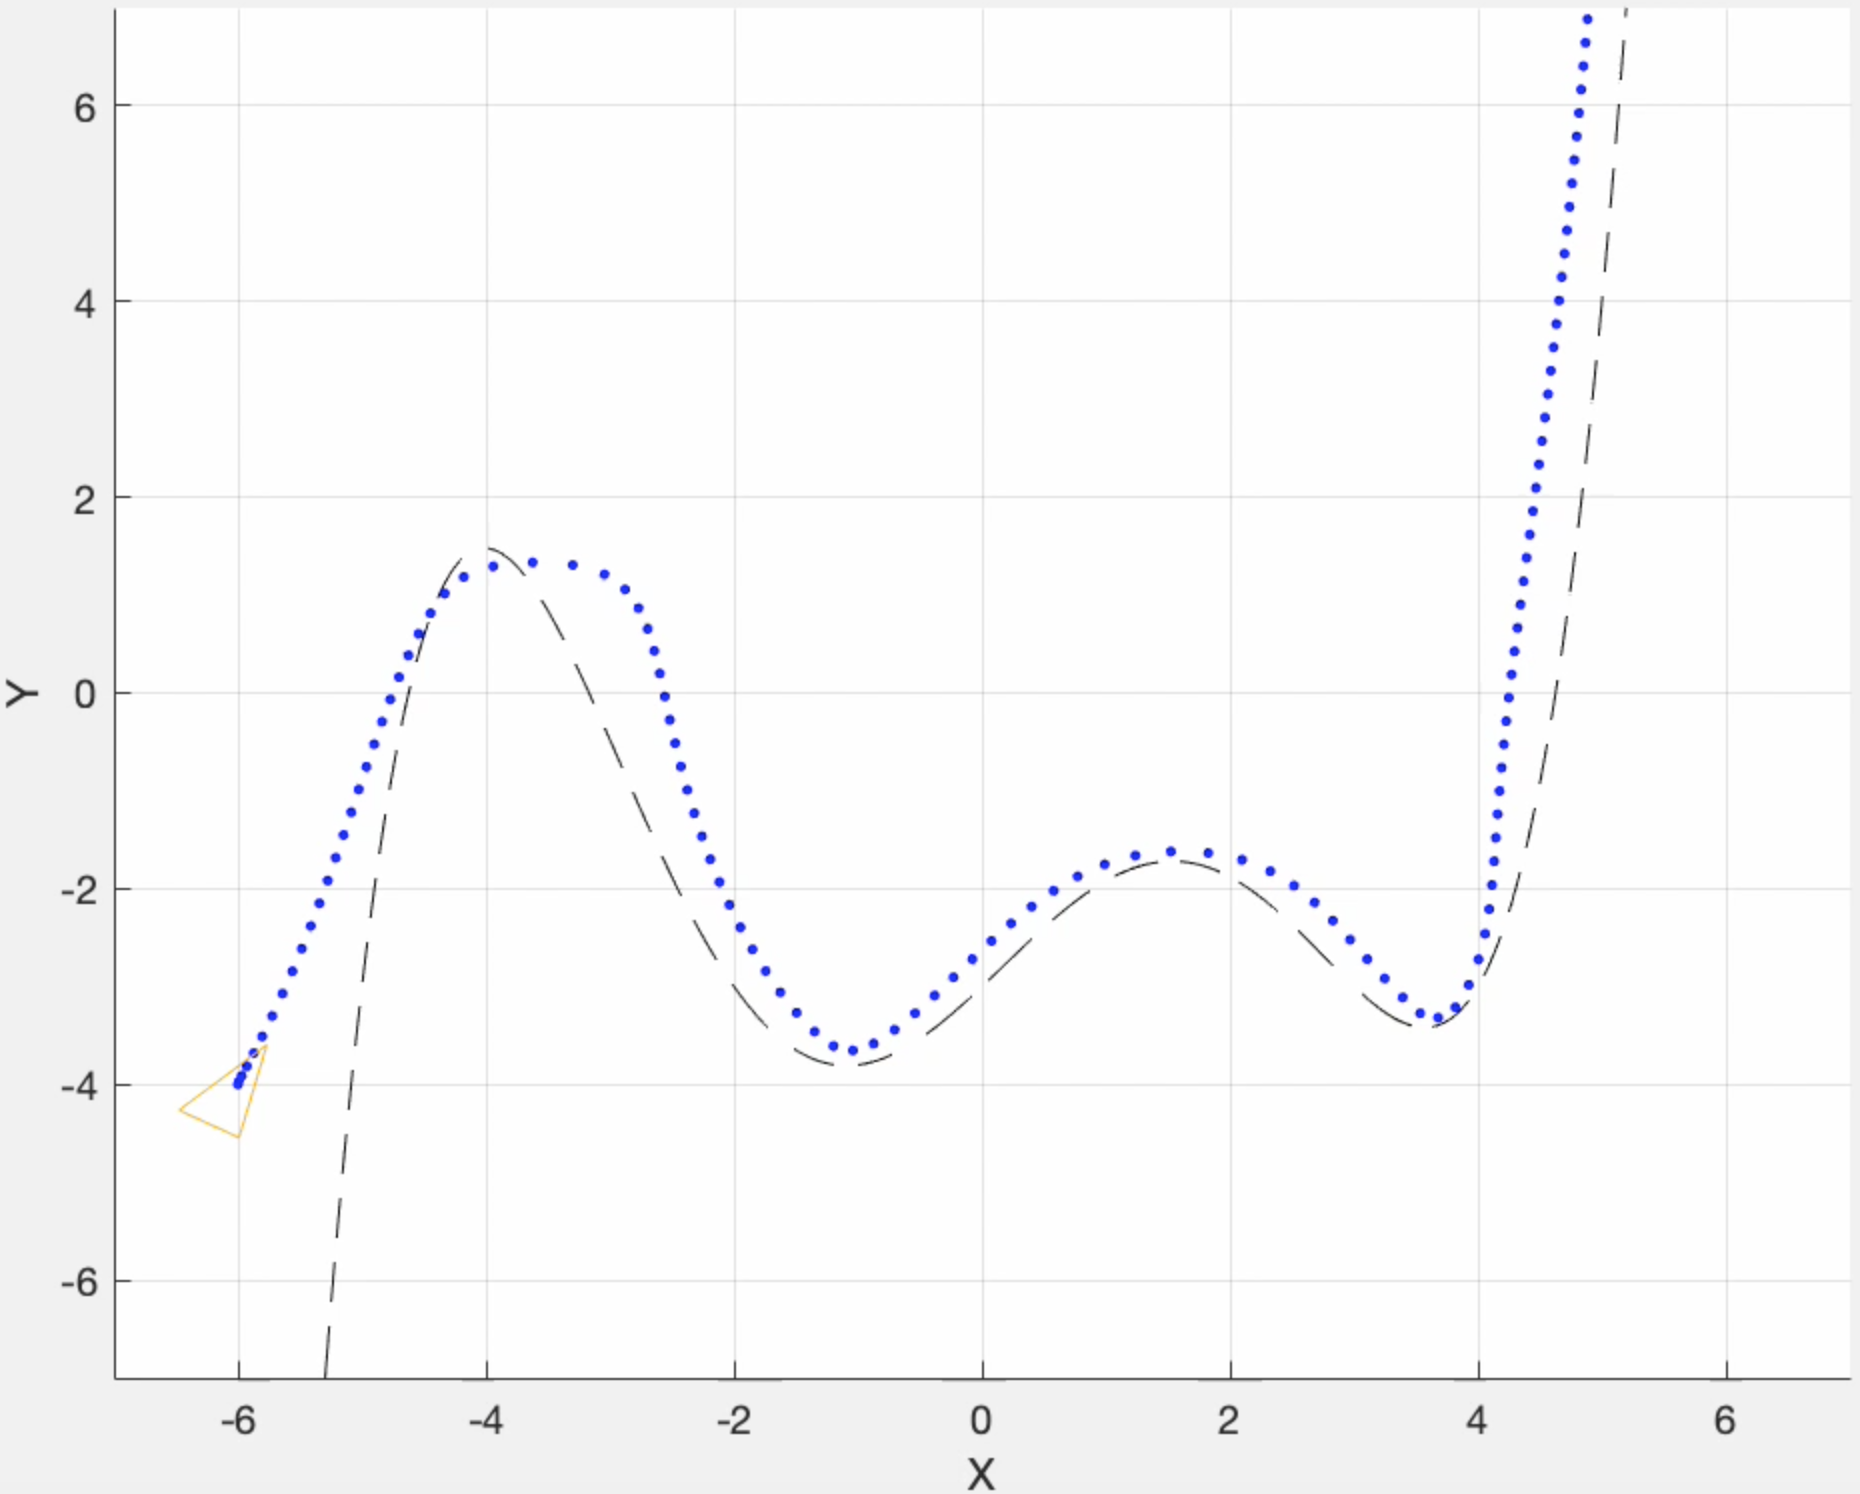
\includegraphics[height=0.3\textheight, width=0.5\textwidth]{images/sim_btm_lft_crn.png}
		\caption{Simulation Plot of Desired Path and Robot Path with Initial Condition $x_3$.}
		\label{fig:sim_btm_lft_crn}
	\end{center}
\end{figure}

The robot in Figure \ref{fig:sim_nr_extr_pth} starts near the first local extrema from the left, and crosses over the desired path. Figure \ref{fig:sim_nr_extr_pth} is a simulation with the almost initial condition as \ref{fig:sim_nr_extr_pth2}; the only difference is $\theta(0)$. The difference in the robot behavior between initial conditions $x_1$ and $x_4$ shows the importance of having a reasonable, with regards to physical constraints, initial condition. Eventually, the robot converges back to the desired path.

\begin{figure}[H]
	\begin{center}
		\includegraphics[height=0.3\textheight, width=0.5\textwidth]{images/sim_nr_extr_pth.png}
		\caption{Simulation Plot of Desired Path and Robot Path with Initial Condition $x_4$.}
		\label{fig:sim_nr_extr_pth}
	\end{center}
\end{figure}

%% Controller Failure
\subsection{Controller Failure}

In this subsection, the initial conditions discussed are
\begin{gather}
    x_5 = \begin{bmatrix} 0 \\ 4 \\ \pi \end{bmatrix} \\
    x_6 = \begin{bmatrix} -4 \\ -5 \\ \frac{\pi}{3} \end{bmatrix}
\end{gather}

Figure \ref{fig:sim_tp_cent} is an example of when the path following controller fails the robot. Due to the nature of distance minimization, there are initial conditions where the robot cannot converge to the desired path because the robot enters a loop where the minimum distance oscillates, leading to movement over the same set of positions.

\begin{figure}[H]
	\begin{center}
		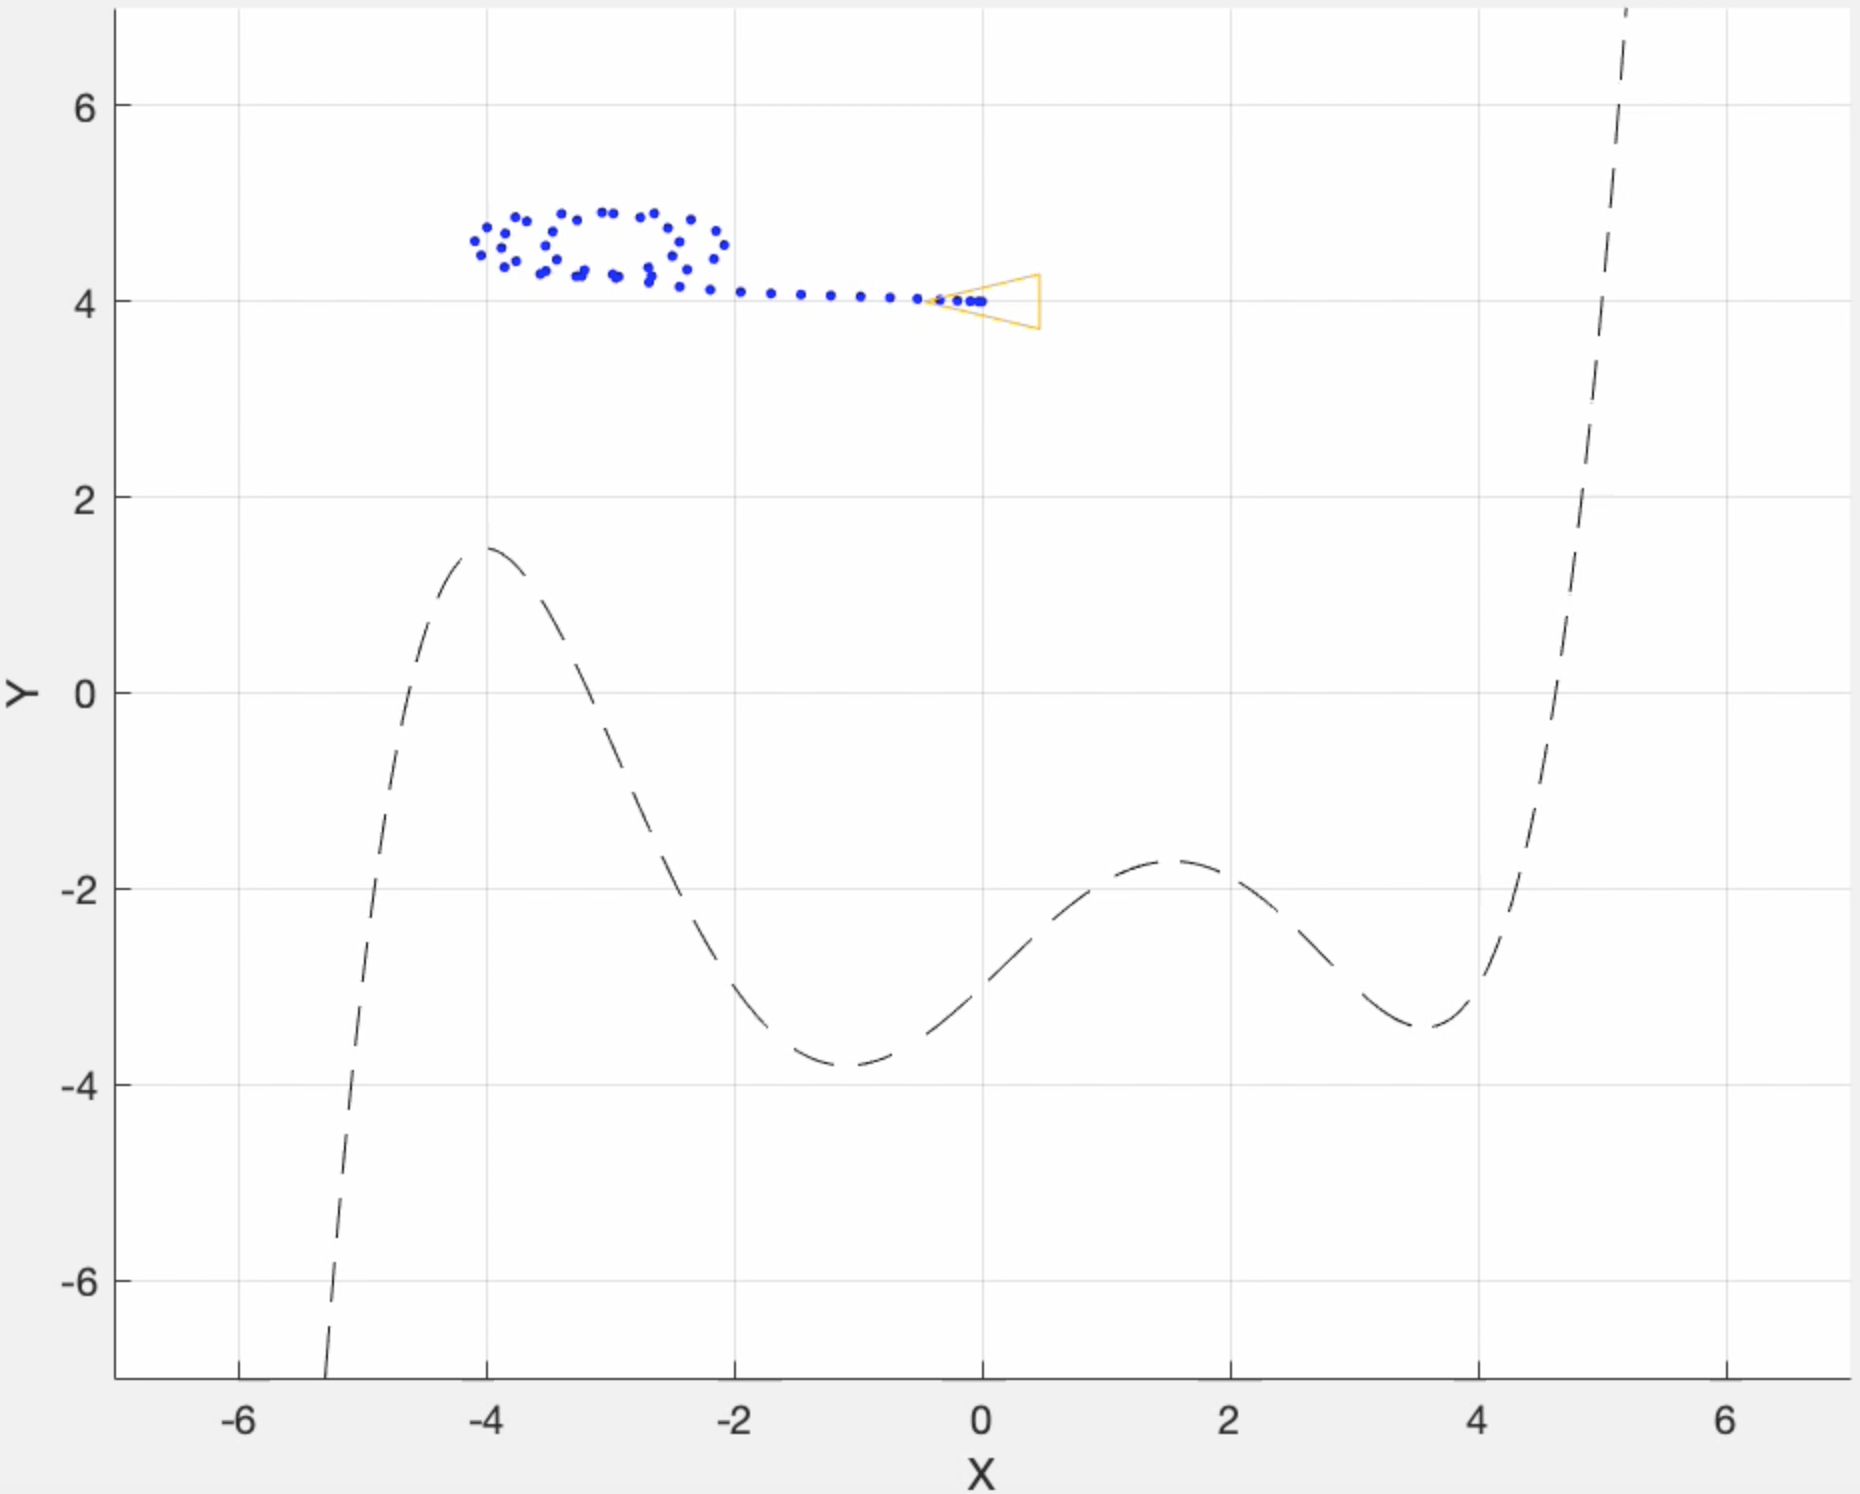
\includegraphics[height=0.3\textheight, width=0.5\textwidth]{images/sim_tp_cent.png}
		\caption{Simulation Plot of Desired Path and Robot Path with Initial Condition $x_5$.}
		\label{fig:sim_tp_cent}
	\end{center}
\end{figure}

\pagebreak

Figure \ref{fig:sim_rgt_pth} is an example that shows the limitations of the path following controller; the path following controller defines the desired path to be on the right side of the robot. The robot in Figure \ref{fig:sim_rgt_pth} attempts to bring the desired path to the right side of the robot, and then converges to the desired path.

\begin{figure}[H]
	\begin{center}
		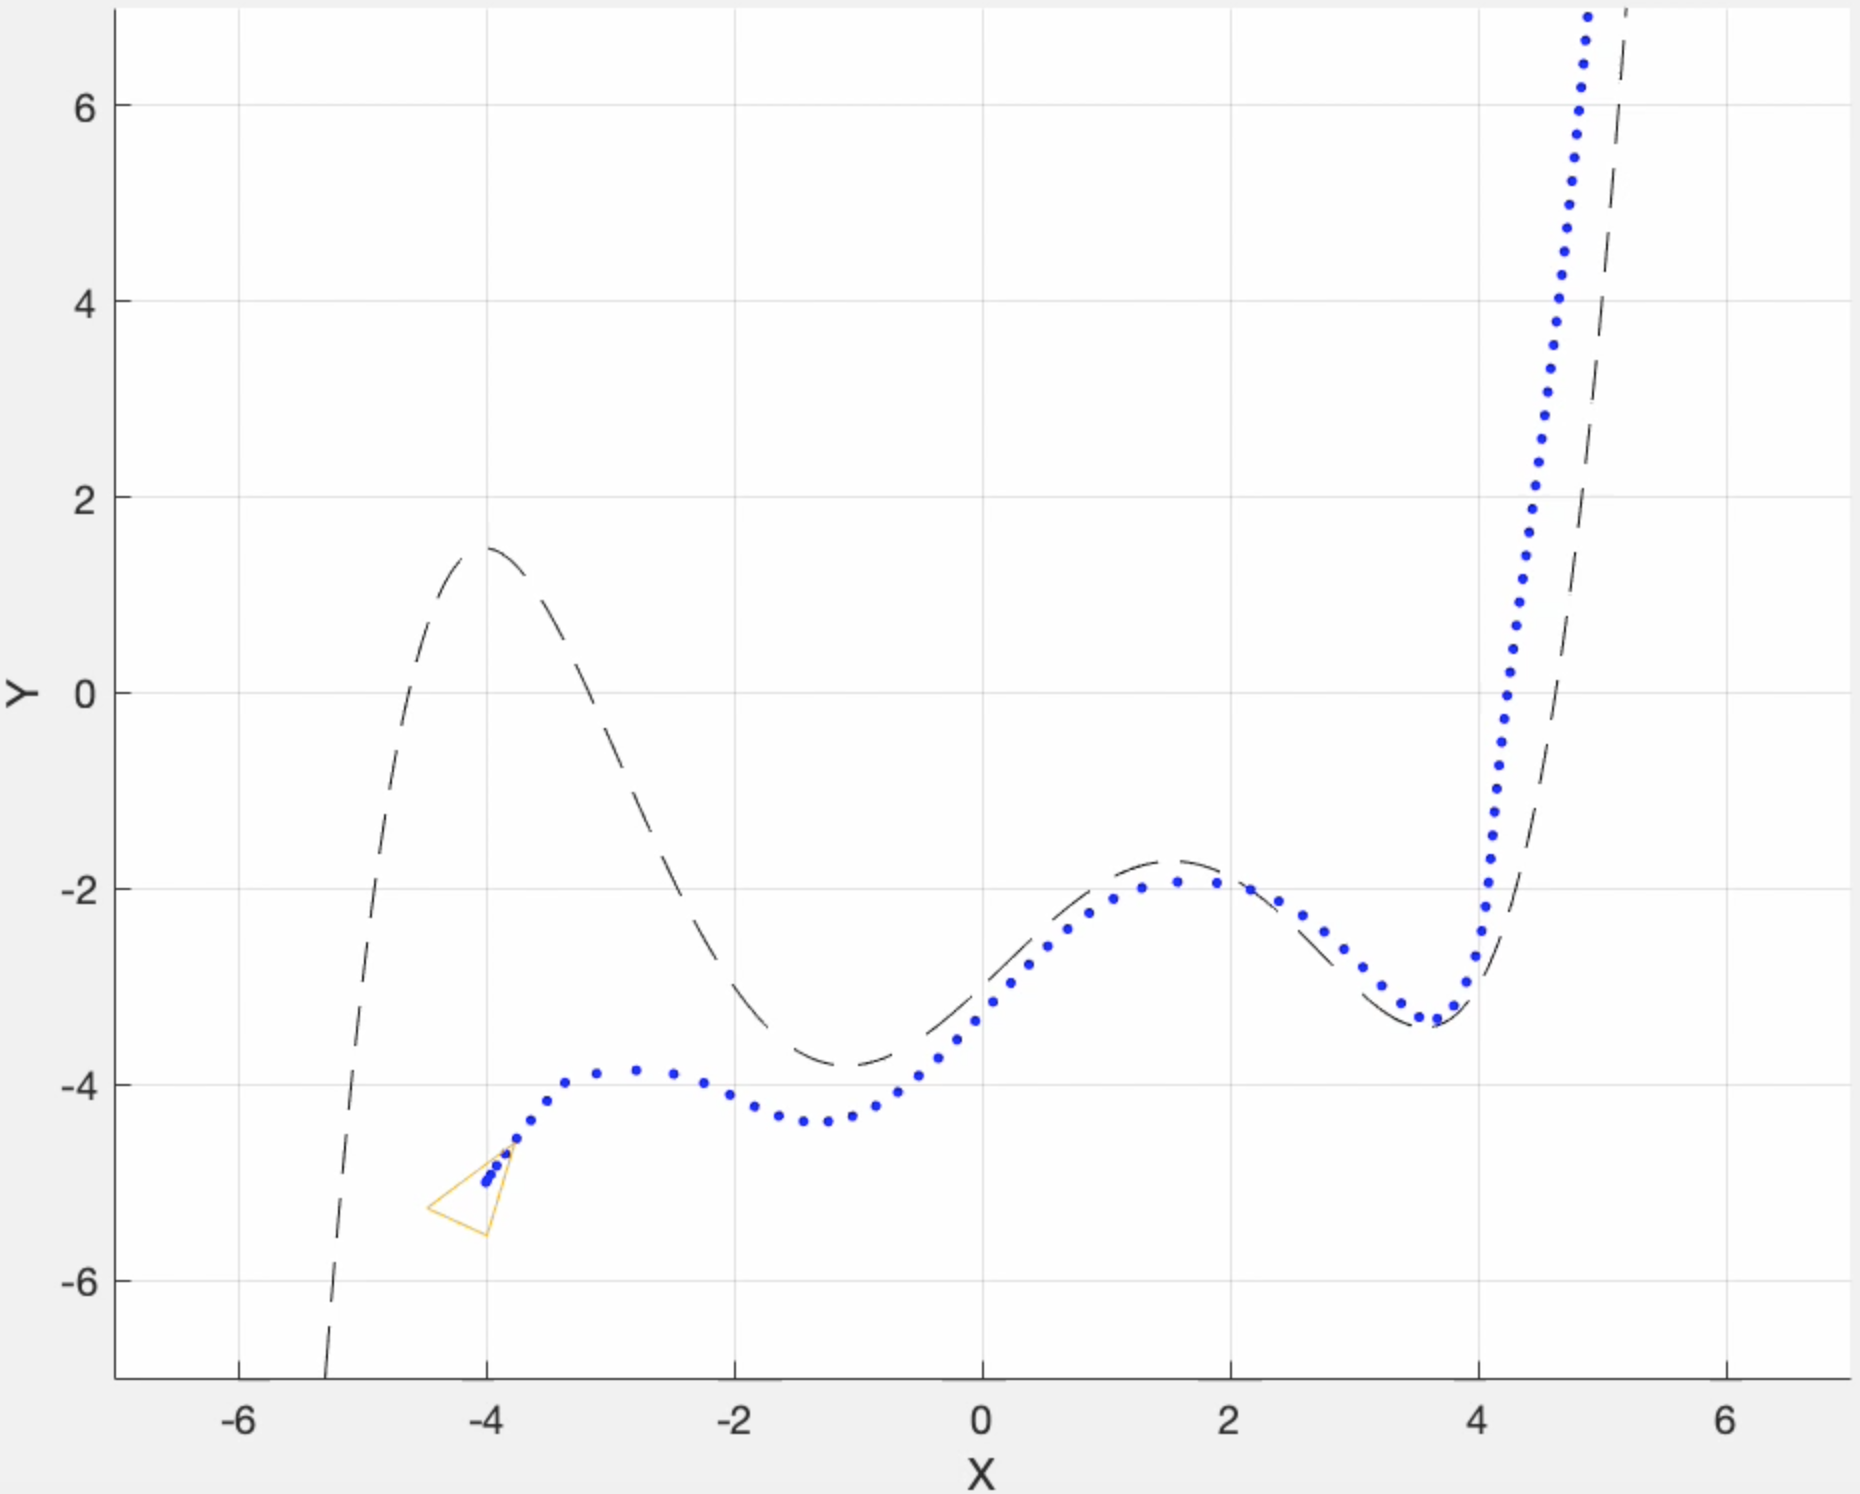
\includegraphics[height=0.3\textheight, width=0.5\textwidth]{images/sim_rgt_pth.png}
		\caption{Simulation Plot of Desired Path and Robot Path with Initial Condition $x_6$.}
		\label{fig:sim_rgt_pth}
	\end{center}
\end{figure}

\end{document}